\documentclass[aspectratio=43,leqno]{beamer}
\usepackage{presentation}
\usetheme{Boadilla}
\setbeamersize
{
  text margin left=.5in,
  text margin right=.5in
}
\usepackage{mathtools}
\usepackage{enumerate}
\usepackage{amssymb}
\usepackage{amsthm}
\usepackage{amsfonts}
\usepackage{xcolor}
\usepackage{fontawesome5}
\usepackage{fontawesome}
\setlength{\parskip}{6pt}
\usepackage{graphicx}
\usepackage{tikz}

\newtheorem{proposition}[theorem]{Proposition}

\newcommand{\R}{\ensuremath{\mathbb{R}}}
\newcommand{\Q}{\ensuremath{\mathbb{Q}}}
\newcommand{\N}{\ensuremath{\mathbb{N}}}
\newcommand{\B}{\ensuremath{\mathcal{B}}}
\newcommand{\X}{\ensuremath{\mathcal{X}}}

\title{\textsc{Spectral Graph Analysis}}
\subtitle{With Applications of Graph Theory in Biological Networks}
\author{Ronald \& Aditya}
\institute{IISER Mohali}

\begin{document}

\begin{frame}
  \titlepage
\end{frame}

\begin{frame}
  \frametitle{Abstract}
  Spectral graph theory can be used to analyze the topological properties (e.g., connectivity) of graphs. Each graph has a Laplacian matrix whose eigenvalues and eigenvectors reveal many properties of the graph. We look at discrete mathematical (graph theoretical) models for biological networks, then study some mathematics of spectral graph theory and in particular, properties of the Laplacian.
\end{frame}

\begin{frame}
  \frametitle{Objectives}
\begin{enumerate}
\item\label{item:1} Take a glimpse at some graph theory models in biology. \pause
\item\label{item:2} Discuss some spectral graph theory and apply it to two biological networks.
\end{enumerate}
\end{frame}

\begin{frame}
  \frametitle{Contents}
\begin{enumerate}
\item Preliminaries: Graph Theory \pause
\item Graph Theory Models in Biological Networks \pause
\item Spectral Graph Theory \pause
\item Two Biological Networks
\begin{itemize}
\item Tissue-specific protein-function associations 
\item Drug-target interaction network
\end{itemize}
\end{enumerate}
\end{frame}

%%%%%%%%%%%%%%%%%%%%%%%%%%%%%%%%%%%%%%%%%%%%%%%%%%%%%%%%%%%%%%%%%%%%%%%%%%
%%%%%%%%%%%% PRELIMS %%%%%%%%%%%%%%%%%%%%%%%%%%%%%%%%%%%%%%%%%%%%%%%%%%%%%
%%%%%%%%%%%%%%%%%%%%%%%%%%%%%%%%%%%%%%%%%%%%%%%%%%%%%%%%%%%%%%%%%%%%%%%%%%

\begin{frame}
  \vfill
\begin{center}
  \textsc{Preliminaries: Graph Theory}
\end{center}
  \vfill
\end{frame}

\begin{frame}
  \frametitle{Preliminaries: Graph Theory}
  \framesubtitle{Degree of a Vertex, a Simple Graph}
  
  A Graph $G = (V, E)$ has set $V$ of vertices and set $E$ of edges connecting the vertices. \pause

  If two vertices $i, j \in V$ are connected by an edge, we write $\{i, j\} \in E$. \pause

  The \emph{degree} of a vertex is the number of edges connected to it. \pause

  A \emph{simple graph} is one where there is at most an edge between any two pair of vertices and there are no self-loops (edges that join the same vertex).
\end{frame}

\begin{frame}
  \frametitle{Preliminaries: Graph Theory}
  \framesubtitle{Types of Graphs}
  
\begin{enumerate}
\item\label{item:6} Undirected graph 
\item\label{item:20} Directed graph (digraph) 
\item\label{item:24} Weighted graph
\end{enumerate}

\end{frame}

\begin{frame}
  \frametitle{Preliminaries: Graph Theory}
  \framesubtitle{Distance}

  The \emph{distance} $\delta(i,j)$ from $i$ to $j$ is the length of the \emph{shortest path} from $i$ to $j$ in $G$. \pause

  The \emph{diameter} of $G$ is the maximum value of $\delta(i, j)$ taken over all distinct pairs of vertices. \pause

  The most common algorithms for calculating the shortest paths are \emph{Dijkstra's} greedy algorithm and \emph{Floyd's} dynamic algorithm.
\end{frame}

%%%%%%%%%%%%%%%%%%%%%%%%%%%%%%%%%%%%%%%%%%%%%%%%%%%%%%%%%%%%%%%%%%%%%%%%%%
%%%%%%%%%%%% GRAPH THEORY MODELS %%%%%%%%%%%%%%%%%%%%%%%%%%%%%%%%%%%%%%%%%
%%%%%%%%%%%%%%%%%%%%%%%%%%%%%%%%%%%%%%%%%%%%%%%%%%%%%%%%%%%%%%%%%%%%%%%%%%

\begin{frame}
  \vfill
\begin{center}
  \textsc{Graph Theory Models in Biological Networks}
\end{center}
  \vfill
\end{frame}

\begin{frame}
  \frametitle{Food Web}
  \framesubtitle{Directed Graph}
  \pause
  
  \begin{figure}[h]
    \centering
    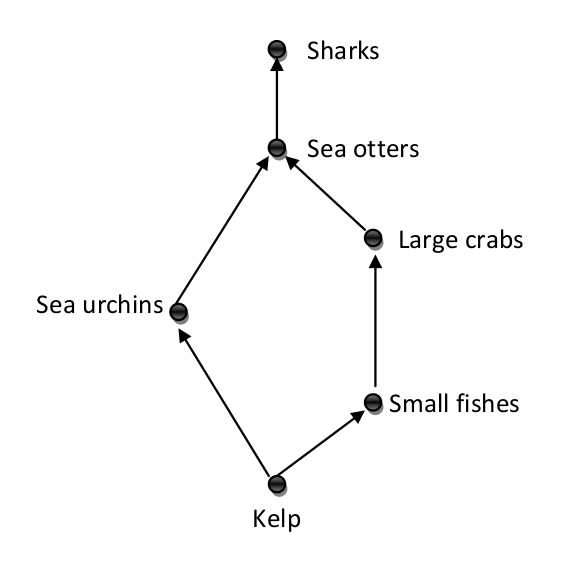
\includegraphics[width=0.5\textwidth]{images/food-web.png}
    \label{fig:mesh1}
  \end{figure}
  \pause
  
\begin{enumerate}
\item\label{item:4} Arrows represent energy flow \pause
\item\label{item:5} Directed graphs represent predator-prey interactions
\end{enumerate}
\end{frame}

\begin{frame}
  \frametitle{Food Web}
  \framesubtitle{Directed Graph}

  We can ask: 
\begin{enumerate}
\item\label{item:7} What are the trophic levels? \pause
\item\label{item:8} What is a dominant species in a food web? \pause 
\item\label{item:9} Can we assign weights to the edges?
\end{enumerate}
\end{frame}

\begin{frame}
  \frametitle{Food Web}
  \framesubtitle{Trophic status}
  
\begin{enumerate}
\item\label{item:10} Two ways to assigning trophic levels: 
\begin{itemize}
\item Shortest path 
\item Longest path \pause
\end{itemize} 
\item\label{item:12} Both of the above methods have shortcomings. \pause
\item\label{item:11} We can define \textbf{trophic status} of a species $u$ by: 
\begin{displaymath}
T(u) = \sum_k^{} kn_k,
\end{displaymath}
where $n_k$ is the number of species whose longest path to $u$ has length $k$.
\end{enumerate} 
\end{frame}

\begin{frame}
  \frametitle{Food Web}
  \framesubtitle{Dominant Species and Weighted Food Webs}
  
\begin{enumerate}
\item\label{item:13} A species is\emph{ dominant} in a food web if its \emph{trophic status} is greater than the number of species in the food web above level $0$. \pause
    \begin{figure}[h]
    \centering
    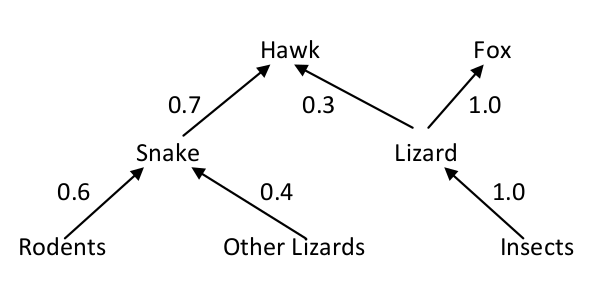
\includegraphics[width=0.5\textwidth]{images/weighted-food-web.png}
    \label{fig:mesh1}
  \end{figure} \pause
\item\label{item:14} We can also define \textbf{flow-based trophic level} (TL) in a weighted food web: 
\begin{displaymath}
\text{TL}(i) = 1 + \sum_i^{} w_{ij} + \text{TL}(\text{food source } j)
\end{displaymath}
\end{enumerate}
  
\end{frame}

\begin{frame}
  \frametitle{Other models}
\begin{enumerate}
\item\label{item:15} Protein-protein interactions (PPI) 
\item\label{item:16} Gene-protein interactions 
\item\label{item:25} Gene regulatory networks (GRN)
\item\label{item:26} Signal transduction networks 
\item\label{item:27} Metabolic and biochemical networks
\end{enumerate}
\end{frame}

%%%%%%%%%%%%%%%%%%%%%%%%%%%%%%%%%%%%%%%%%%%%%%%%%%%%%%%%%%%%%%%%%%%%%%%%%
%%%%%%%%%%% SPECTRAL GRAPH THEORY %%%%%%%%%%%%%%%%%%%%%%%%%%%%%%%%%%%%%%%
%%%%%%%%%%%%%%%%%%%%%%%%%%%%%%%%%%%%%%%%%%%%%%%%%%%%%%%%%%%%%%%%%%%%%%%%%

\begin{frame}
  \vfill
\begin{center}
 \textsc{Spectral Graph Theory}
\end{center}
  \vfill
\end{frame}

\begin{frame}
  \frametitle{From Graphs to Matrices}
  \framesubtitle{Adjacency Matrix}
  
\begin{center}
\begin{tikzpicture}
\draw (0,0) node[anchor=north east]{$2$} -- (1.5,2.6) node[anchor=south]{$1$}-- (3,0) node[anchor=north west]{$3$}-- cycle;
\filldraw[black] (0,0) circle (1.5pt);
\filldraw[black] (1.5,2.6) circle (1.5pt);
\filldraw[black] (3,0) circle (1.5pt);
\end{tikzpicture}
\begin{displaymath}
  \begin{pmatrix} 0 & 1 & 1 \\
    1 & 0 & 1 \\
    1 & 1 & 0
  \end{pmatrix}
\end{displaymath}
\end{center}
  The graph and the matrix has the same information.
\end{frame}

\begin{frame}
  \frametitle{From Graphs to Matrices}
  \framesubtitle{Adjacency Matrix}
  
\begin{definition}[Adjacency matrix]
  The adjacency matrix $A \in \{0,1\}^{n\times n}$ is defined by 
\begin{displaymath}
A_{ij} =
\begin{cases}
  1 & \text{if }\{i, j\} \in E, \\
  0 & \text{otherwise}.
\end{cases}
\end{displaymath} 
\end{definition}
\pause
 
\begin{enumerate}
\item\label{item:17} $A$ is symmetric for an undirected graph. 
\item\label{item:18} $A$ has diagonal elements zero if there are no self-loops.
\end{enumerate}
\pause

\begin{definition}[Degree matrix]
  The degree matrix $D \in \mathbb{R}^{n\times n}$ is defined as the diagonal matrix with diagonal entries $(d_1, \ldots, d_n)$. 
\end{definition}

\end{frame}

\begin{frame}
  \frametitle{From Graphs to Matrices}
  \framesubtitle{Normalized adjacency matrix}
\begin{definition}[Normalized adjacency matrix]
  The normalized adjacency matrix is defined by $\overline{A} = AD^{-1}$.
\end{definition}
\pause

\begin{enumerate}
\item\label{item:19} $\overline{A}$ is not necessarily symmetric. But it is column-stochastic, that is, each column has nonnegative entries that sum to $1$. \pause
\item\label{item:21} Suppose $\rho \in \mathbb{R}^n$ is a probability distribution, $\overline{A}\rho$ is another probability distribution. Therefore, we have a \emph{random walk} on the graph!
\end{enumerate}

\end{frame}

\begin{frame}
  \frametitle{From Graphs to Matrices}
  \framesubtitle{Laplacian matrix}
  
\begin{definition}[Laplacian matrix]
  The Laplacian matrix is defined as $L = D - A$.
\end{definition}
\pause

\begin{definition}[Normalized Laplacian matrix]
  The normalized Laplacian matrix is defined as 
\begin{displaymath}
\overline{L} = D^{-1/2}LD^{-1/2} = \mathbb{I} - D^{-1/2}AD^{-1/2}.
\end{displaymath}
\end{definition}
\end{frame}

\begin{frame}
  \frametitle{From Graphs to Matrices}
  \framesubtitle{Laplacian matrix}
  
\begin{enumerate}
\item\label{item:22} $L$ and $\overline{L}$ are always symmetric. \pause
\item\label{item:23} They are best thought of as quadratic forms: for any $x\in \mathbb{R}^n$, 
\begin{displaymath}
x^T L x = \sum_i d_ix_i^2 - \sum_{(i,j)\in E} x_ix_j = \sum_{\{i,j\}\in E} (x_i-x_j)^2.
\end{displaymath}
\end{enumerate}

\end{frame}

\begin{frame}
  \frametitle{From Graphs to Matrices}
  \framesubtitle{Normalized Laplacian matrix}

\begin{proposition}
  $\forall x \in \mathbb{R}^n$, we have 
\begin{displaymath}
x^T \overline{L} x = \sum_{\{i,j\}\in E} \left( \frac{x_i}{\sqrt{d_i}} - \frac{x_j}{\sqrt{d_j}} \right)^2.
\end{displaymath} 
\end{proposition}
\pause

If $G$ is $d$-regular, then this simplifies to 
\begin{displaymath}
x^T\overline{L}x = \frac{1}{d} \sum_{\{i,j\}\in E} (x_i-x_j)^2.
\end{displaymath}

\end{frame}

\begin{frame}
  \frametitle{Eigenvalues and Eigenvectors of the Laplacian}
  \framesubtitle{A single edge}

\begin{center}
\begin{tikzpicture}
  \draw (0,0) -- (2,0);
  \filldraw[black] (0,0) circle(1.5pt);
  \filldraw[black] (2,0) circle(1.5pt);
\end{tikzpicture}
\end{center}
  The adjacency matrix and degree matrix are
\begin{displaymath}
A = \begin{pmatrix} 0 & 1 \\ 1 & 0 \end{pmatrix} \text{ and } D = \begin{pmatrix} 1 & 0 \\ 0 & 1 \end{pmatrix}.
\end{displaymath}
\pause

The Laplacians are 
\begin{displaymath}
L = \begin{pmatrix} 1 & -1 \\ -1 & 1 \end{pmatrix} = \overline{L}.
\end{displaymath}
\pause

The eigenvalues of $\overline{L}$ are given by $\lambda_1 = 0, \lambda_2 = 2$ whose corresponding eigenvectors are 
\begin{displaymath}
\frac{1}{\sqrt{2}} \begin{pmatrix} 1 \\ 1 \end{pmatrix} \text{ and } \frac{1}{\sqrt{2}} \begin{pmatrix} 1 \\ -1 \end{pmatrix}.
\end{displaymath}

\end{frame}

\begin{frame}
  \frametitle{Eigenvalues and Eigenvectors of the Laplacian}
  \framesubtitle{A triangle graph}
\begin{displaymath}
  A = \begin{pmatrix} 0 & 1 & 1 \\ 1 & 0 & 1 \\ 1 & 1 & 0 \end{pmatrix},
  \text{ and }
  D = \begin{pmatrix} 2 & 0 & 0 \\ 0 & 2 & 0 \\ 0 & 0 & 2 \end{pmatrix}.
\end{displaymath}
\pause

The Laplacian matrix is 
\begin{displaymath}
  L = \begin{pmatrix} 1 & -1/2 & -1/2 \\ -1/2 & 1 & -1/2 \\ -1/2 & -1/2 & 1 \end{pmatrix}. 
\end{displaymath}
\pause

The eigenvalues of $\overline{L}$ are $\{ 0, 3/2, 3/2 \}$ with corresponding eigenvectors
\begin{displaymath}
  \frac{1}{\sqrt{3}} \begin{pmatrix} 1 \\ 1 \\ 1 \end{pmatrix},
  \frac{1}{\sqrt{6}} \begin{pmatrix} 2 \\ -1 \\ -1 \end{pmatrix},
  \frac{1}{\sqrt{2}} \begin{pmatrix} 0 \\ 1 \\ -1 \end{pmatrix}.
\end{displaymath}

\end{frame}

\begin{frame}
    \frametitle{Eigenvalues and Eigenvectors of the Laplacian}
    \framesubtitle{The path of length 2}

\begin{displaymath}
  A = \begin{pmatrix} 0 & 1 & 0 \\ 1 & 0 & 1 \\ 0 & 1 & 0 \end{pmatrix},
  \text{ and }
  D = \begin{pmatrix} 1 & 0 & 0 \\ 0 & 2 & 1 \end{pmatrix}.
\end{displaymath}
\pause

The Laplacian matrix is 
\begin{displaymath}
L = \begin{pmatrix} 1 & -1/\sqrt{2} & 0 \\ -1/\sqrt{2} & 1 & -1/\sqrt{2} \\ 0 & -1/\sqrt{2} & 1 \end{pmatrix}.
\end{displaymath}
\pause

The eigenvalues of $\overline{L}$ are $\{ 0, 1, 2 \}$ with corresponding eigenvectors 
\begin{displaymath}
  \frac{1}{2} \begin{pmatrix} 1 \\ \sqrt{2} \\ 1 \end{pmatrix}, \frac{1}{\sqrt{2}} \begin{pmatrix} -1 \\ 0 \\ 1 \end{pmatrix}, \frac{1}{2} \begin{pmatrix} -1 \\ \sqrt{2} \\ -1 \end{pmatrix}.
\end{displaymath}

\end{frame}

\begin{frame}
    \frametitle{Eigenvalues of the Laplacian}

\begin{proposition}
For any graph $G$ with normalized Laplacian $\overline{L}$, if $\lambda_1$ is the smallest eigenvalue of $\overline{L}$ then $\lambda_1 = 0$ with multiplicity equal to the number of connected components of $G$.
\end{proposition}
\pause

\begin{corollary}
For any graph $G$, the second smallest eigenvalue $\lambda_2(\overline{L})>0$ if and only if $G$ is connected.
\end{corollary}
\end{frame}

\begin{frame}
  \frametitle{The Laplacian}
  \framesubtitle{Properties}

  For an undirected graph $G$ and its Laplacian matrix $\overline{L}$ with eigenvalues 
\begin{displaymath}
0 = \lambda_1 \leq \lambda_2 \leq \cdots \leq \lambda_{n}:
\end{displaymath} 
\begin{itemize}
\item\label{item:3} $\overline{L}$ is positive-semidefinite (that is, $\lambda_i \geq 0$). \pause 
\item\label{item:28} Every row sum and column sum of $\overline{L}$ is zero. \pause
\item\label{item:29} The second smallest nonzero eigenvalue of $\overline{L}$ (could be zero) is the algebraic connectivity (or Fiedler value) of $G$. \pause
\item The trace of the Laplacian matrix $\overline{L}$ is equal to $2m$ where $m$ is the number of edges of the considered graph.
\end{itemize}
\end{frame} 

\begin{frame}
  \frametitle{Graph Connectivity}
  \framesubtitle{Using Eigenvalues of the Laplacian}

  The second smallest eigenvalue $\lambda_2$ tells us about the connectivity of the graph. \pause
\begin{enumerate}
\item\label{item:31} If $G$ has two disconnected components, $\lambda_2 = 0$. \pause
\item\label{item:32} If $\lambda_2$ is small, this suggests the graph is nearly disconnected. \pause
\item\label{item:33} In short, $\lambda_2$ gives us a sort of continuous measure of how well a graph is connected.
\end{enumerate}
\end{frame}

%%%%%%%%%%%%%%%%%%%%%%%%%%%%%%%%%%%%%%%%%%%%%%%%%%%%%%%%%%%%%%%%%%%%%%%%
%%%%%%%%%% TWO BIOLOGICAL SYSTEMS %%%%%%%%%%%%%%%%%%%%%%%%%%%%%%%%%%%%%%
%%%%%%%%%%%%%%%%%%%%%%%%%%%%%%%%%%%%%%%%%%%%%%%%%%%%%%%%%%%%%%%%%%%%%%%%

\begin{frame}
  \vfill
\begin{center}
  \textsc{Two Biological Systems}
\end{center}
  \vfill
\end{frame}

\begin{frame}
  \frametitle{Protein-function associations}
  \framesubtitle{Tissue-specific protein-function associations}

  This is a collection of protein-function association networks for a large number of human tissues. Nodes represent human proteins, tissues, and biological functions. Edges represent associations that indicate different biological roles of proteins in various tissues and cell types.

\end{frame}

\begin{frame}
  \frametitle{Protein-function associations}
  \framesubtitle{Tissue-specific protein-function associations}

    \begin{figure}[h]
    \centering
    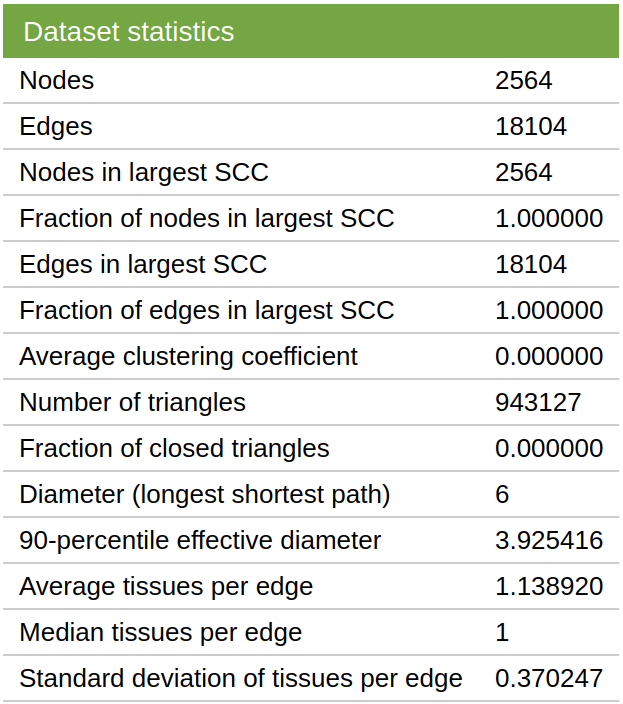
\includegraphics[width=0.5\textwidth]{images/tfg.png}
    \label{fig:mesh1}
  \end{figure}
  
\end{frame}

\begin{frame}
  \frametitle{Protein-function associations}
  \framesubtitle{Tissue-specific protein-function associations}

    \begin{figure}[h]
    \centering
    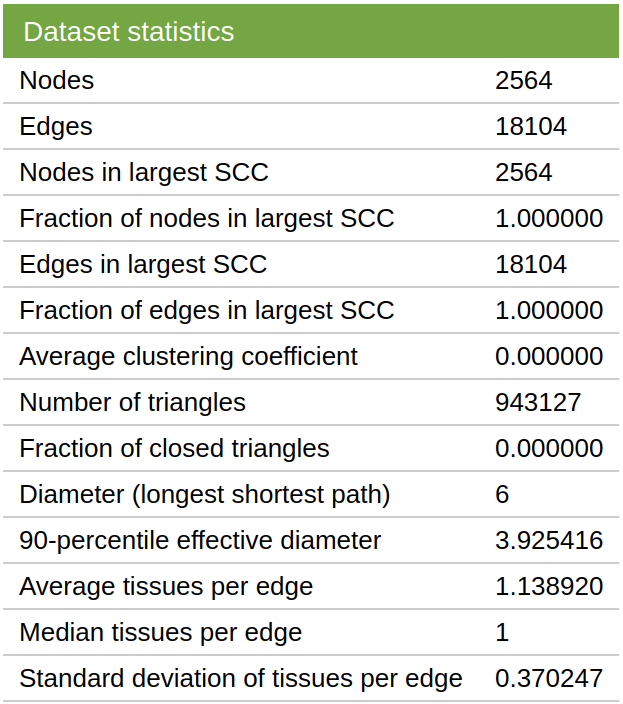
\includegraphics[width=0.5\textwidth]{images/tfg.png}
    \label{fig:mesh1}
  \end{figure}
  
\end{frame}

\begin{frame}
  \frametitle{Protein-function associations}
  \framesubtitle{Code on GitHub}

 \begin{figure}[h]
    \centering
    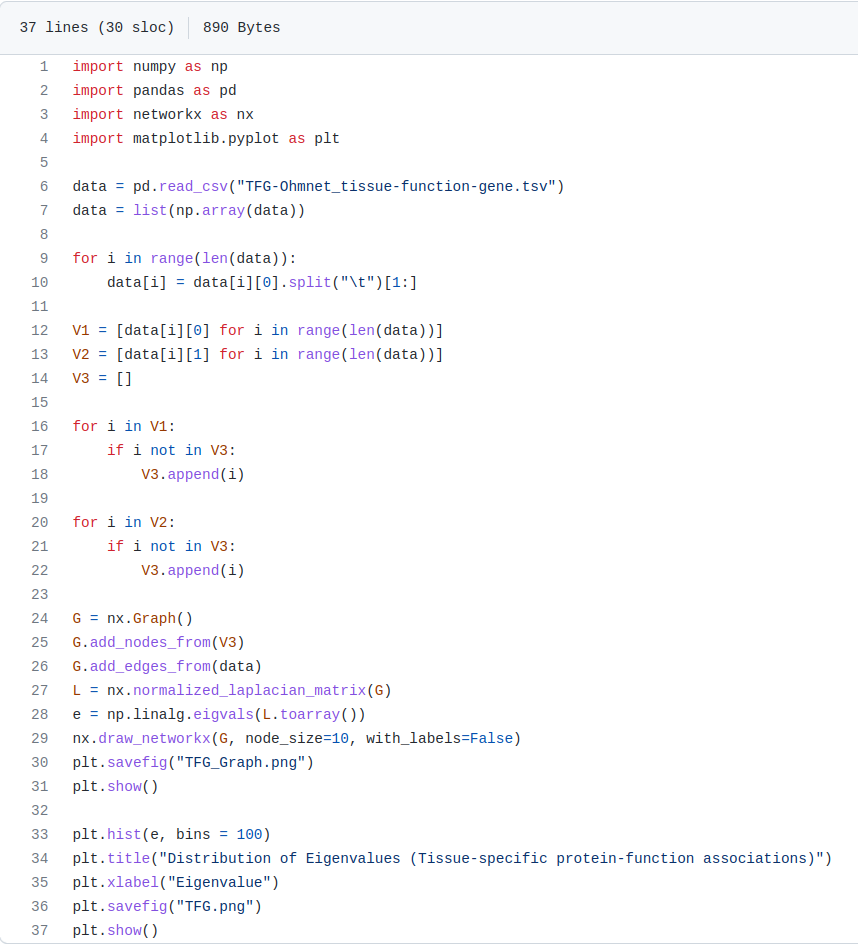
\includegraphics[width=0.5\textwidth]{images/tfg-code.png}
    \label{fig:mesh1}
  \end{figure}
  \hyperref{https://github.com/huidr/spectral-graph-analysis/tfg.py}{}{}{https://github.com/huidr/spectral-graph-analysis/tfg.py}
  
\end{frame}

\begin{frame}
  \frametitle{Protein-function associations}
  \framesubtitle{Plotting the Graph}

 \begin{figure}[h]
    \centering
    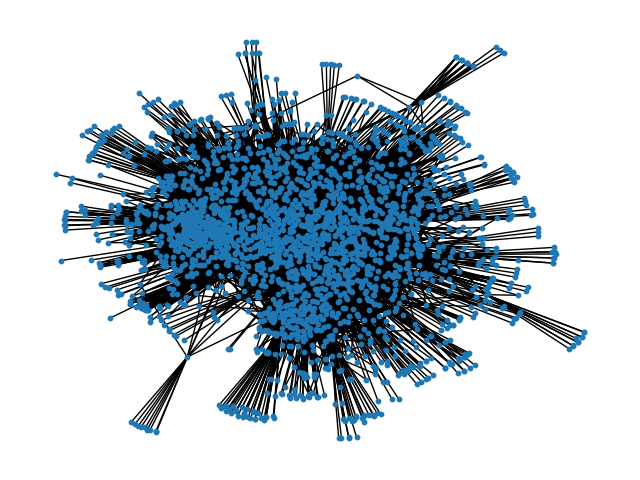
\includegraphics[width=0.8\textwidth]{images/tfg-graph.png}
    \label{fig:mesh1}
  \end{figure}
  
\end{frame}

\begin{frame}
  \frametitle{Protein-function associations}
  \framesubtitle{Plotting the Histogram of the Eigenvalues}

 \begin{figure}[h]
    \centering
    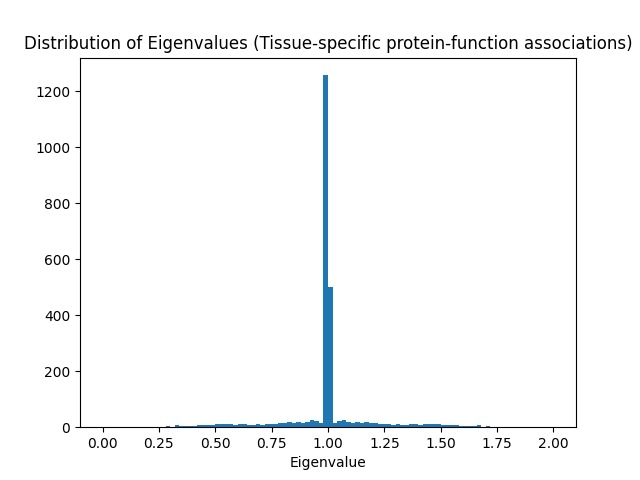
\includegraphics[width=0.9\textwidth]{images/tfg-hist.jpeg}
    \label{fig:mesh1}
  \end{figure}
  
\end{frame}


\begin{frame}
  \frametitle{Drug-target interaction network}
  
This is a drug-target interaction network that contains information on which genes (i.e., proteins encoded by genes) are targeted by drugs that are on the U.S. market. Drug targets are molecules that play a critical role in the transport, delivery or activation of the drug. 

\end{frame}

\begin{frame}
  \frametitle{Drug-target interaction network}
  
    \begin{figure}[h]
    \centering
    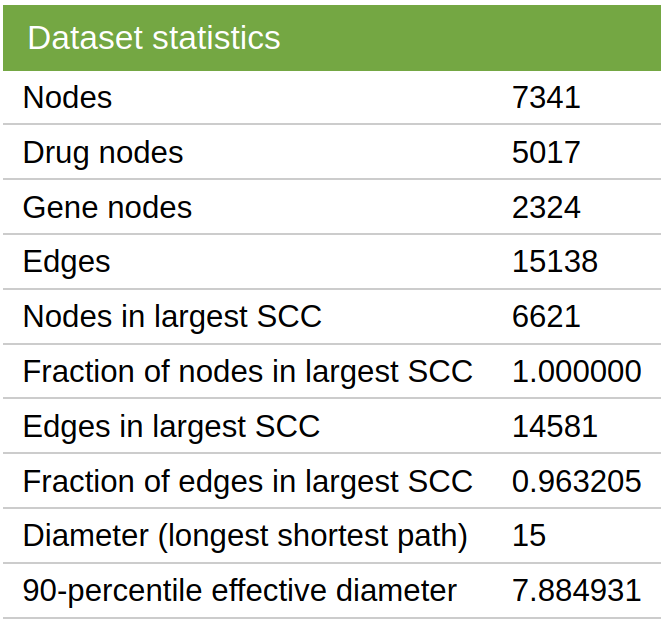
\includegraphics[width=0.5\textwidth]{images/chg.png}
    \label{fig:mesh1}
  \end{figure}
  
\end{frame}

\begin{frame}
    \frametitle{Drug-target interaction network}
  \framesubtitle{Code on GitHub}

 \begin{figure}[h]
    \centering
    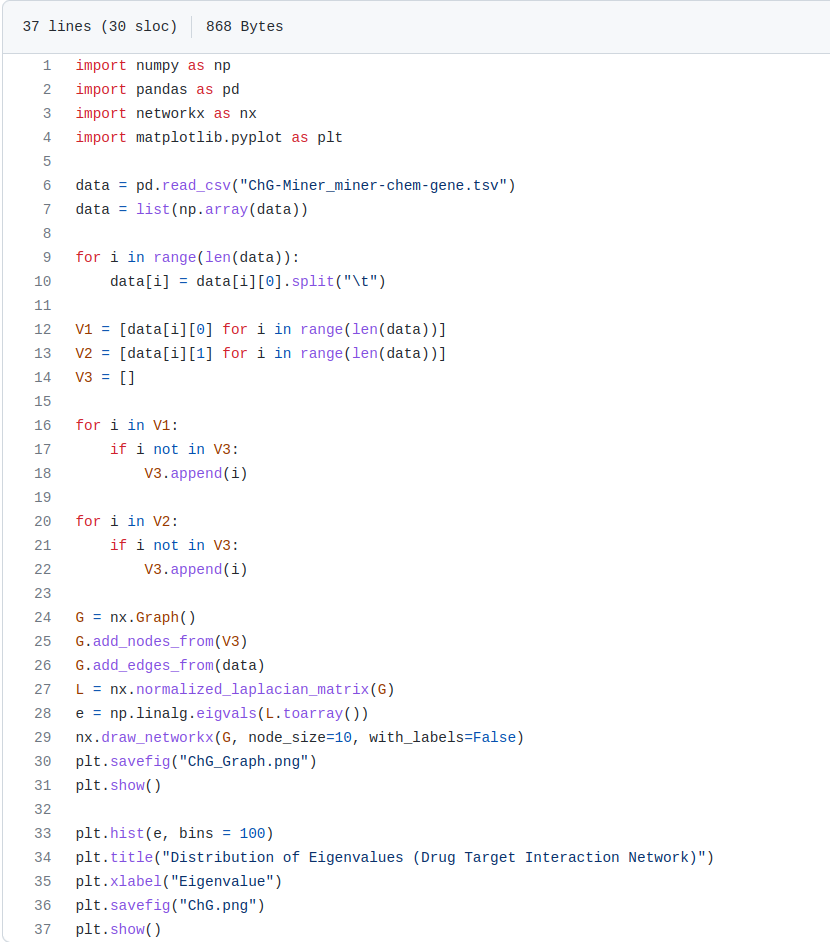
\includegraphics[width=0.5\textwidth]{images/chg-code.png}
    \label{fig:mesh1}
  \end{figure}
  \hyperref{https://github.com/huidr/spectral-graph-analysis/tfg.py}{}{}{https://github.com/huidr/spectral-graph-analysis/chg.py}
  
\end{frame}

\begin{frame}
    \frametitle{Drug-target interaction network}
  \framesubtitle{Plotting the Graph}

 \begin{figure}[h]
    \centering
    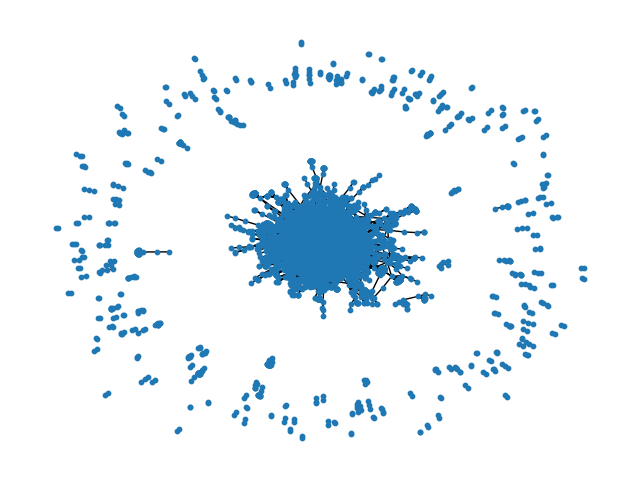
\includegraphics[width=0.8\textwidth]{images/chg-graph.png}
    \label{fig:mesh1}
  \end{figure}
  
\end{frame}

\begin{frame}
    \frametitle{Drug-target interaction network}
  \framesubtitle{Plotting the Histogram of the Eigenvalues}

 \begin{figure}[h]
    \centering
    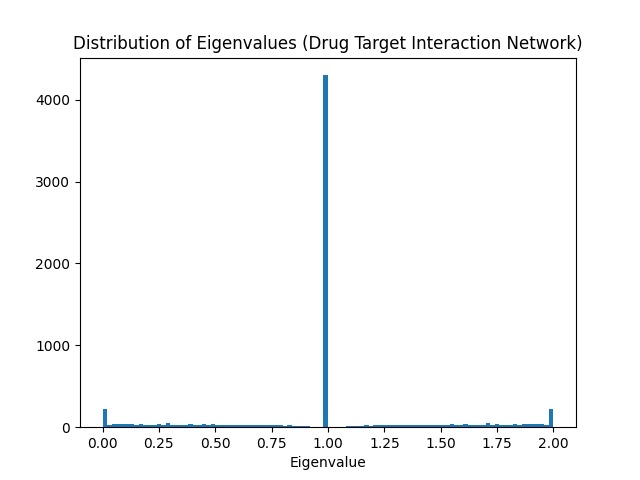
\includegraphics[width=0.9\textwidth]{images/chg-hist.jpeg}
    \label{fig:mesh1}
  \end{figure}
  
\end{frame}

\begin{frame}
  \vfill
  The dataset of the two biological networks we used are available at:

  {\color{blue} \hyperref{https://snap.stanford.edu/biodata/}{}{}{https://snap.stanford.edu/biodata/} }
  \vfill
\end{frame}

\begin{frame}

  \vfill
  All of our work is on GitHub.
  
  {\color{blue} \hyperref{https://github.com/huidr/spectral-graph-analysis}{}{}{https://github.com/huidr/spectral-graph-analysis} }

  \vfill
  
\end{frame}

%%%%%%%%%%%%%%%%%%%%%%%%%%%%%%%%%%%%%%%%%%%%%%%%%%%%%%%%%%%%%%%%%%%%%%%%
%%%%%%%%%%% REFERENCES %%%%%%%%%%%%%%%%%%%%%%%%%%%%%%%%%%%%%%%%%%%%%%%%%
%%%%%%%%%%%%%%%%%%%%%%%%%%%%%%%%%%%%%%%%%%%%%%%%%%%%%%%%%%%%%%%%%%%%%%%%

\begin{frame}
  \frametitle{References}

  \begin{thebibliography}{1}
  \bibitem[]{} M. Cozzens. \emph{Food Webs, Competition Graphs, and Habitat Formation}. Math. Model. Nat. Phenom., Vol. 6, No. 6, 2011, pp. 22-38.
  \end{thebibliography}

  \begin{thebibliography}{1}
  \bibitem[]{} Introduction to Spectral Graph Theory. \hyperref{http://users.cms.caltech.edu/~vidick/notes/CMS139/spectral.pdf}{}{}{http://users.cms.caltech.edu/~vidick/notes/CMS139/spectral.pdf}
  \end{thebibliography}

\end{frame}
\end{document}